\documentclass{article}
\usepackage[utf8]{inputenc}
\usepackage[cm]{fullpage}
%\usepackage[]{geometry}
\usepackage[]{graphicx}
\usepackage[]{listings}
\usepackage{rotating}
\usepackage{amsmath}
\usepackage{circuitikz}
\usepackage{titlesec}
\usepackage{latexsym}
% \usepackage{enumerate}
\usepackage{enumitem}
\usepackage{amsmath,amsfonts,amsmath,amssymb}
\newcommand{\HRule}{\rule{\linewidth}{0.5mm}}
\usepackage[colorlinks,pagebackref,pdfusetitle,urlcolor=blue,citecolor=blue,bookmarksnumbered,plainpages=false]{hyperref}

\titleformat{\section}
  {\normalfont\Large\bfseries}{\thesection}{1em}{}[{\titlerule[0.8pt]}]
  
\begin{document}

\begin{titlepage}
\begin{center}

\textsc{\LARGE Oregon State University}\\[1.5cm]

\textsc{\Large Computational Complexity (Theory of Computation) - CS 517}\\[0.5cm]

% Title
\HRule \\[0.4cm]
{ \huge \bfseries Final Project (Draft)\\[0.4cm] }

\HRule \\[1.5cm]

% Author and supervisor
\noindent
\begin{minipage}{0.4\textwidth}
\begin{flushleft} \large
\emph{Student:}\\
Ben \textsc{McCamish}
\end{flushleft}
\end{minipage}%
\begin{minipage}{0.4\textwidth}
\begin{flushright} \large
\emph{Professor:} \\
Mike \textsc{Rosulek}\\
\emph{TA:} \\
Naimisha \textsc{Saireddy}
\end{flushright}
\end{minipage}

\vfill

% Bottom of the page
%{\large May 20, 2019}

\end{center}
\end{titlepage}

\section{Introduction}
Most users do not know the structure and content of databases and concepts such as schema or formal query languages sufficiently well to express their information needs precisely in the form of queries~\cite{Usable:Jagadish,Chen:2009:KSS,Idreos:SIGMOD:2015}. They may convey their intents in easy-to-use but inherently ambiguous forms, such as keyword queries, which are open to numerous interpretations. Thus, it is very challenging for a database management system (DBMS) to understand and satisfy the intents behind these queries. The fundamental challenge in the interaction of these users and DBMS is that the users and DBMS represent intents in different forms.

Many such users may explore a database to find answers for various intents over a rather long period of time. For these users, database querying is an inherently interactive and continuing process. As both the user and DBMS have the same goal of the user receiving her desired information, the user and DBMS would like to gradually improve their understandings of each other and reach a {\it common language of representing intents} over the course of various queries and interactions. The user may learn more about the structure and content of the database and how to express intents as she submits queries and observes the returned results. Also, the DBMS may learn more about how the user expresses her intents by leveraging user feedback on the returned results. The user feedback may include clicking on the relevant answers \cite{Yue:2012:KDB:2240304.2240501}, the amount of time the user spends on reading the results \cite{Granka:2004:EAU:1008992.1009079}, user's eye movements \cite{Huang:2012:USU:2207676.2208591}, or the signals sent in touch-based devises \cite{DBLP:conf/icde/LiarouI14}. Ideally, the user and DBMS should establish as quickly as possible this common representation of intents in which the DBMS accurately understands all or most user's queries.

Researchers have developed systems that leverage user feedback to help the DBMS understand the intent behind ill-specified and vague queries more precisely \cite{Chaudhuri:2006:PIR:1166074.1166085,Chatzopoulou:2009:QRI:1561638.1561642}. These systems, however, generally assume that a user does {\it not} modify her method of expressing intents throughout her interaction with the DBMS. For example, they maintain that the user picks queries to express an intent according to a fixed probability distribution. It is known that the learning methods that are useful in a static setting do not deliver desired outcomes in a setting where all agents may modify their strategies \cite{Grotov:2016:OLR:2911451.2914798,Daskalakis:2010:LAN:1929237.1929248}. Hence, one may not be able to use current techniques to help the DBMS understand the users' information need in a rather long-term interaction.

\section{Framework}
\label{sec:framework}
We have modeled this interaction between the user and the DBMS as an interactive game. The user will first start by selecting some intent. Then they choose a query to represent that intent and send it to the DBMS. The DBMS, upon receiving this query, will determine what tuple it should return to the user. 

\subsection{User Strategy}
The user begins their interaction by considering what intent to communicate to the DBMS. An intent is the information that the user is seeking from the DBMS. However, the user may not know how to express this intent in such a way that the DBMS can understand what they are seeking. A user unfamiliar with the DBMS structure, content, or query language, may use keyword queries to interact with a DBMS. For example, if the user was searching a database of colleges, they might be searching for ``Oregon State University''. To express this intent, they may send the keyword query ``OSU''. Keyword queries can be translated into some structured query language such as SQL. However, for this project we will be referring to queries as keyword queries. For the sake of this project the specific query language does not matter beyond examples.

Thus, the user has a strategy that maps their intents, what they are searching for, to the set of possible queries they can use to express that intent. This mapping is a row stochastic mapping. The user can learn and update their strategy overtime using common reinforcement learning algorithm techniques~\cite{roth1995learning,cross1973stochastic,bush1953stochastic,cen2013reinforcement}. Thus, overtime the user can learn to communicate effectively with the DBMS their intents. This may take quite a long amount of time, but it eventually will happen. In practice, a user has finitely many intents and submits finitely many queries in a finite period of time. Hence, we assume that the sets of the user's intents and queries are finite. We index each user's intent and query by $1 \leq i \leq m$ and $1 \leq j \leq n$, respectively. A user strategy, denoted as $U$, is a $m\times n$ row-stochastic matrix from her intents to her queries. 

\subsection{DBMS Strategy}
The DBMS receives keyword queries from the user and must decide how to respond with tuples. A naive approach would be to simply return all the tuples that have the keyword(s) received ranked using some popular ranking algorithm such as BM25~\cite{robertson2009probabilistic}. This requires that the user knows some keywords that might possibly return results. This also relies on the ranking algorithm to effectively return the correct tuple high enough in the results such that the user is able to view it. 

In our model we take another approach. The DBMS has a strategy that given a keyword query, it responds with some probability with a tuple. This can trivially be extended for the case of returning multiple tuples by either sampling multiple times or returning tuple sets. For now, we will focus on the case where the DBMS only returns a single tuple. The DBMS can also learn and update its strategy overtime using the same reinforcement learning algorithms that the user might use. It can also use other popular algorithms such as UCB-1~\cite{auer2002finite,vorobev2015gathering, radlinski2008learning, moon2012online}. The DBMS strategy is represented for a user as an $n\times o$ row-stochastic matrix from the set of the user's queries to the set of possible tuples to return. We index each query and tuple by $1 \leq j \leq n$ and $1 \leq l \leq o$. Each pair of the user and the DBMS strategy, ($U$,$D$), is a {\it strategy profile}. The expected payoff for both players with strategy profile ($U$,$D$) is as follows.

\begin{align}
\label{eqn:payoff}
u_{r}(U,D) =\sum_{i=1}^m\pi_i\sum_{j=1}^nU_{ij}\sum_{\ell=1}^o D_{jl}\ r, 
\end{align}

\subsection{Overview}
The overall view is the user considers an intent to search the DBMS for and picks a query to send, based on their strategy $U$. The DBMS receives that query and returns some tuple, based on its strategy $D$.  In Equation~\ref{eqn:payoff} $\pi$ is the prior probability that a user will search for some intent $i$. The reward $r$ then becomes whether the tuple received by the user matches their intent. Of course, more complicated reward metrics may be used such as Precision, Recall, NDCG, or MRR~\cite{IRStyle,IRBook}. However, for this project we will simply restrict it to the case of ``did the user receive the tuple or not'', thus a boolean reward of either 0 or 1. The user may later decide to query for another intent with a different signal. The DBMS might later decide to return a different tuple upon receiving the same query. However, both of the players in this game share the payoff since the goal of both the user and the DBMS is the same, to return a tuple that matches the user's intent.

\subsection{Equilibria}
Our game model uses one similar to the one presented in Game Theory, called a Signaling Game~\cite{Cho:QuarterlyJournalEconomics:1987,hu2011reinforcement}. This game is founded on the idea that one agent sends signals to another and that agent decides how it should respond to that signal. Each agent can adjust their strategies overtime and eventually reach a point where they are communicating to some degree effectively. In fact, they are communicating to such a degree that any change to the current strategy by either player would reduce the current payoff they are receiving, or a ``stable state''. Payoff in this case is shown in Equation~\ref{eqn:payoff}. The range for the payoff values are [0,1].

This ``stable state'' is called a Nash equilibria. A Nash equilibria is defined as a state in which neither player can unilaterally deviate from their current strategy and receive a higher payoff. Another definition is for a Strict Nash equilibria in which neither player can unilaterally deviate from their current strategy and receive the \textit{same} or higher payoff. There are also instances of either \textit{pure} or \textit{mixed} Nash equilibria. A pure Nash equilibria means that each strategy is deterministic in which actions are taken given an observation of the other players action. A mixed strategy has some probability associated with whether a given action will take place~\cite{10.2307/1969529}.

It has been proved that there is always a mixed Nash equilibria in a game~\cite{10.2307/1969529}. However, there may not be a pure Strict Nash equilibria. In general, finding a mixed Nash equilibria is not NP-Complete, but instead in a special class called PPAD-Complete~\cite{daskalakis2009complexity}. With certain restrictions to the problem, however, it has been shown to be NP-Complete~\cite{gilboa1989nash,sandholm2002complexity}. One such property is when the game is played in such a way that the agents share their payoff. This is the case for our model of the game. 

\section{Reduction}
\label{sec:reductions}
We will be reducing and creating three main contributions, of which the reductions are showing Sections~\ref{sec:payoff}, \ref{sec:strictnash}, and~\ref{sec:nash}. The other portions of Section~\ref{sec:reductions} are required to ensure that the solution falls within the bounds of our game. You might say they contain the supporting clauses for the SMT.

\subsection{Simplifications}
\label{sec:simplifications}
We will be making some simplifications to our model. We are restricting the strategies to only Pure Strategies, thus only probabilities of 0 or 1 in strategies. After our discussion and emailing the student you put me in contact with, we couldn't find a way to construct a bounded quantifier for the reductions. SMT is also limited in that all variables in the formula must have the same domain. Since we are using a uniform prior over the intents we are left with fractions in Equation~\ref{eqn:payoff}. Thus all variables in the following reductions are Real numbers.

We will be instantiating some of the reductions for clarity. For these instantiations, we will use the strategy profile and reward matrix in Figure~\ref{example:framework:table:strategies:sender}, \ref{example:framework:table:strategies:receiver}, and \ref{example:framework:table:strategies:reward}. We will also be using notation such that the variable $U_{apple,x}$ is the variable for that cell in the user strategy. In addition, we will be showing each part of the reduction separately. The final SMT will of course be a conjunction between the individual portions, but it should be clearer by breaking them up into separate parts. 

\begin{table}[h!]
	\centering
    \begin{minipage}{.2\linewidth}
        \caption{User strategy}
        \centering
        \begin{tabular}{c|c|c|}
            \cline{2-3}
             & \multicolumn{1}{c|}{$x$} & $y$\\
            \hline
            \multicolumn{1}{|c|}{``CS''} & 0 & 1\\
            \hline
            \multicolumn{1}{|c|}{``EE''} & 1 & 0\\
            \hline
        \end{tabular}
        \label{example:framework:table:strategies:sender}
    \end{minipage}
    \begin{minipage}{.35\linewidth}
        \caption{DBMS strategy}
        \centering
        \begin{tabular}{c|c|c|}
            \cline{2-3}
             & \multicolumn{1}{c|}{``CS517''} & ``EE533''\\
            \hline
            \multicolumn{1}{|c|}{$x$} & 0 & 1\\
            \hline
            \multicolumn{1}{|c|}{$y$} & 1 & 0\\
            \hline
        \end{tabular}
        \label{example:framework:table:strategies:receiver}
    \end{minipage}
       \begin{minipage}{.3\linewidth}
        \caption{Reward Matrix}
        \centering
        \begin{tabular}{c|c|c|}
            \cline{2-3}
             & \multicolumn{1}{c|}{``CS517''} & ``EE533''\\
            \hline
            \multicolumn{1}{|c|}{``CS''} & 1 & 0\\
            \hline
            \multicolumn{1}{|c|}{``EE''} & 0 & 1\\
            \hline
        \end{tabular}
        \label{example:framework:table:strategies:reward}
    \end{minipage}
\end{table}

\subsection{Domains}
The first clause in the reduction will be that of the domains for each variable. Since the strategies we are looking at are Pure strategies, then the variables can only take on values 0 and 1. Due to some of the limitations of SMT, each of the variables are real numbers. Thus, to enforce this restriction, we have the following SMT:

\begin{align}
\label{eqn:domain}
&(U_{1,1} = 0\lor U_{1,1} = 1)\land(U_{1,2} = 0\lor U_{1,2} = 1)\land\ldots\land(U_{m,n} = 0\lor U_{m,n} = 1)\\
\land&(D_{1,1} = 0\lor D_{1,1} = 1)\land(D_{1,2} = 0\lor D_{1,2} = 1)\land\ldots\land(D_{n,o} = 0\lor D_{n,o} = 1)\nonumber
\end{align}

As a reminder, $n$ is the number of intents, $m$ is the number of queries, and $o$ is the number of tuples to return. This makes sure that any variables that would be assigned a value in an accepting equilibria will have either a 0 or 1 value. We won't show an example for this, as it takes up quite a bit of space.

\subsection{Stochastic}
With only the domain reduction, it would be possible to get strategies with 1s in every cell. However, our model uses row stochastic matrices. The SMT to ensure that each strategy is row stochastic is as follows:

\begin{align}
\label{eqn:stochastic}
&(U_{1,1} + U_{1,2} + \ldots + U_{1,m}=1)\land(U_{2,1} + U_{2,2} + \ldots + U_{2,m}=1)\land\ldots\land(U_{n,1} + U_{n,2} + \ldots + U_{n,m}=1)\\
\land&(D_{1,1} + D_{1,2} + \ldots + D_{1,o}=1)\land(D_{2,1} + D_{2,2} + \ldots + D_{2,o}=1)\land\ldots\land(D_{n,1} + D_{n,2} + \ldots + D_{n,o}=1)\nonumber
\end{align}

Using the example in Section~\ref{sec:simplifications}, we would have the following:
\begin{align}
\label{eqn:stochastic:example}
&(U_{CS,x} + U_{CS,y}=1)\land(U_{EE,x} + U_{EE,y}=1)\land(D_{x,CS517} + D_{x,EE433}=1)\land(D_{y,CS517} + D_{y,EE433}=1)
\end{align}

Since the sum of all rows now is equal to 1, an assignment of variables to our strategies will be stochastic.

\subsection{Payoff}
\label{sec:payoff}
One portion of this project is to see if there is a strategy that can achieve some minimum amount of payoff. The following reduction is how we can ensure that any assignments to the variables must have a minimum payoff using Equation~\ref{eqn:payoff}. Not all sets of intents, queries, and tuples will be able to achieve all payoffs, thus depending on the setting and the minimum required payoff, no such assignment may exist.

\begin{align}
\label{eqn:payoffreduction}
(\pi_1U_{1,1}D_{1,1}R_{1,1} + \pi_1U_{1,1}D_{1,2}R_{1,2} + \ldots + \pi_2U_{2,1}D_{1,1}R_{2,1} + \ldots + \pi_mU_{m,n}D_{n,o}R_{m,o}) \ge MinPayoff
\end{align}

Of course, this could easily be changed such that we want a payoff of exactly some value, then we could change the inequality to be that of an equals. Using the example in Section~\ref{sec:simplifications}, we would have the following:

\begin{align}
\label{eqn:payoffreduction:example}
&\pi_{CS}U_{CS,x}D_{x,CS517}R_{CS,CS517} + \pi_{CS}U_{CS,x}D_{x,EE433}R_{CS,EE433} +\\\nonumber
&\pi_{CS}U_{CS,y}D_{y,CS517}R_{CS,CS517} + \pi_{CS}U_{CS,y}D_{y,EE433}R_{CS,EE433}+\\\nonumber
&\pi_{EE}U_{EE,x}D_{x,CS517}R_{EE,CS517} + \pi_{EE}U_{EE,x}D_{x,EE433}R_{EE,EE433} +\\\nonumber
&\pi_{EE}U_{EE,y}D_{y,CS517}R_{EE,CS517} + \pi_{EE}U_{EE,y}D_{y,EE433}R_{EE,EE433}\\\nonumber
=&0.5\cdot0\cdot0\cdot1 + 0.5\cdot0\cdot1\cdot0 + 0.5\cdot1\cdot1\cdot1 + 0.5\cdot1\cdot0\cdot0+\\\nonumber
&0.5\cdot1\cdot0\cdot0 + 0.5 \cdot1\cdot1\cdot1 + 0.5\cdot0\cdot1\cdot0 + 0.5\cdot0\cdot0\cdot1\\\nonumber
=&1\\\nonumber
\end{align}

We can see that the current strategy we have in the example is the highest payoff possible in this strategy. However, we by making some changes we can see the payoff change. For example if the DBMS instead returned ``CS517'' for both queries $x$ and $y$, the payoff would then be 0.5. 

\subsection{Nash Equilibria}
\label{sec:nashequil}
In order for the assignment of variables to be in either a Strict Nash or Nash equilibria, we need to add to the SMT some inequalities that capture unilateral deviations from the current strategy. A unilateral deviation is where one player changes their strategy while the other player's remains the same. For instance, using the example in Section~\ref{sec:simplifications}, a unilateral deviation would be if the user instead sent query $y$ for ``CS'' instead of $x$ and the DBMS strategy remained the same. 

To perform this reduction, we need a strategy for every single cell in both strategies. For the current example that would be 8 strategies. We will refer to these as \textit{Nash Strategies}. A Nash Strategy is slightly different from the regular strategy. It duplicates the regular strategies variables in every way, including the domain and stochastic restrictions with one exception. It introduces new variables for a single row. The row must remain stochastic and each new variable in that row will have the same domain restrictions. One of these new variables will also have the added restriction that it cannot equal the current strategy. Thus we have the SMT as follows, where $NU_{x,y,j,k}$ is the Nash strategy for the user for the $x$ row and $y$ column. $j$ and $k$ are the cells within that strategy. The same is true for the DBMS side with $ND_{x,y,j,k}$. We denote $NU$ and $ND$ with separate notation indicating which player is unilaterally deviating from their strategy to clarify the reduction. However, it should be noted that all reductions described here apply to either $NU$ or $ND$.

\begin{align}
\label{eqn:nasheq}
&(NU_{1,1,1,1} \ne U_{1,1}) \land (NU_{1,2,1,2} \ne U_{1,2})\land\ldots\land(NU_{n,m,n,m}\ne U_{n,m})\\
&\land(ND_{1,1,1,1} \ne D_{1,1}) \land (ND_{1,2,1,2} \ne D_{1,2})\land\ldots\land(ND_{m,o,m,o}\ne D_{m,o}))\nonumber
\end{align}

The notation for this is confusing, so let's look at the example strategy in Section~\ref{sec:simplifications} again. The current user strategy variables are shown in Table~\ref{example:regular}. The variables for the Nash User Strategy for the first row and first column are in Table~\ref{example:nash11}. The variables for the Nash User Strategy for the first row and second column are in Table~\ref{example:nash12}.

\begin{table}[h!]
    \centering
    \begin{minipage}{.2\linewidth}
        \caption{User strategy}
        \centering
        \begin{tabular}{|c|c|}
            \hline
            $U_{CS,x}$ & $U_{CS,y}$\\
            \hline
            $U_{EE,x}$ & $U_{EE,y}$\\
            \hline
        \end{tabular}
        \label{example:regular}
    \end{minipage}
    \begin{minipage}{.3\linewidth}
        \caption{Nash User strategy 1,1}
        \centering
        \begin{tabular}{|c|c|}
            \hline
            $NU_{1,1,CS,x}$ & $NU_{1,1,CS,y}$\\
            \hline
            $U_{EE,x}$ & $U_{EE,y}$\\
            \hline
        \end{tabular}
        \label{example:nash11}
    \end{minipage}
    \begin{minipage}{.3\linewidth}
        \caption{Nash User strategy 1,2}
        \centering
        \begin{tabular}{|c|c|}
            \hline
            $NU_{1,2,CS,x}$ & $NU_{1,2,CS,y}$\\
            \hline
            $U_{EE,x}$ & $U_{EE,y}$\\
            \hline
        \end{tabular}
        \label{example:nash12}
    \end{minipage}
\end{table}

Using the SMT above and the two Nash Strategies in Tables~\ref{example:nash11} and~\ref{example:nash12}, we would have the following:

\begin{align}
\label{eqn:nashexample}
(NU_{1,2,CS,y} \ne U_{CS,y}) \land (NU_{1,1,CS,x} \ne U_{CS,x})
\end{align}

Notice that we do not have any restrictions on $NU_{1,2,CS,x}$ and $NU_{1,1,CS,y}$. If we had a strategy that had three queries for example, then if we put restrictions on those variables it would be impossible to find a satisfying assignment as 2 of the variables would have to be 0. At least one of those two would already be 0 in the User strategy, since the strategies are row stochastic. It is also enough to simply say that the Nash User Strategy cell is not equal to the User Strategy cell since the only values they can possess are 0 or 1. Thus, all possible moves from the current strategy will represented by these new variables. 

To get an idea of how many new variables we are introducing, consider again the example. We have 8 new Nash Strategies, each of which are introducing new variables for every column. Thus we have $8\cdot2=16$ new variables, where only 8 of those variables have the above restriction. All 16 have the domain restriction. All 8 of the strategies also have the stochastic restriction. Both of these follow the same reduction as done previously. Consider the Nash Strategy variables in Table~\ref{example:nash11} again. We would add to the SMT the following:

\begin{align}
(NU_{1,1,CS,x} + NU_{1,1,CS,y}=1)\land(NU_{1,1,CS,x}=0 \lor NU_{1,1,CS,x}=1)\land(NU_{1,1,CS,y}=0 \lor NU_{1,1,CS,y}=1)
\end{align}

Each of these new Nash Strategies also has some payoff, which is calculated the same as the normal one. Consider again the Nash User Strategy in Table~\ref{example:nash11}. The payoff function for this would be as follows:

\begin{align}
\label{eqn:payoffreductionnash:example}
&\pi_{CS}NU_{1,1,CS,x}D_{x,CS517}R_{CS,CS517} + \pi_{CS}NU_{1,1,CS,x}D_{x,EE433}R_{CS,EE433} +\\\nonumber
&\pi_{CS}NU_{1,1,CS,y}D_{y,CS517}R_{CS,CS517} + \pi_{CS}NU_{1,1,CS,y}D_{y,EE433}R_{CS,EE433}+\\\nonumber
&\pi_{EE}U_{EE,x}D_{x,CS517}R_{EE,CS517} + \pi_{EE}U_{EE,x}D_{x,EE433}R_{EE,EE433} +\\\nonumber
&\pi_{EE}U_{EE,y}D_{y,CS517}R_{EE,CS517} + \pi_{EE}U_{EE,y}D_{y,EE433}R_{EE,EE433}\\\nonumber
\end{align}

Note that only the two new variables are introduced into the payoff. This is because we only want to check the payoff after a single move. That is to say, we want to know the payoff after changing a row such that is not equal to the original row.

\subsection{Pure Strict Nash Equilibria Reduction}
\label{sec:strictnash}
For the reduction to an SMT that will produce a Strict Nash Equilibria if one exists, we take all the Nash Strategies created in Section~\ref{sec:nashequil} and make sure that their payoff is less than the original strategy payoff. To simplify the notation we will be representing the Nash User Strategy Payoff for the cell $x,y$, as $NUP_{x,y}$. One example of this formula is in~Equation\ref{eqn:payoffreductionnash:example}. The DBMS movements will be similar with notation $NDP_{x,y}$. The original payoff will be represented as $P$. The reduction would then be as follows:

\begin{align}
\label{eqn:strictnash}
&(NUP_{1,1} < P) \land (NUP_{1,2} < P) \land \ldots\land (NUP_{n,m} < P)\\
&\land(NDP_{1,1} < P) \land (NDP_{1,2} < P) \land \ldots\land (NDP_{m,o} < P)
\end{align}

Since this is a Strict Nash equilibria, each of the moves that any player can make must have a strictly smaller payoff then the current one.

\subsection{Pure Nash Equilibria Reduction}
\label{sec:nash}
A Nash equilibria will always exist. However, a Strict Nash equilibria may not. Reduction for a Nash Equilibria is very similar. Instead we adjust the inequality to instead allow for strategies that have the same payoff as follows:

\begin{align}
\label{eqn:nash}
&(NUP_{1,1} \le P) \land (NUP_{1,2}\le P) \land \ldots\land (NUP_{n,m} \le P)\\
&\land(NDP_{1,1} \le P) \land (NDP_{1,2} \le P) \land \ldots\land (NDP_{m,o} \le P)
\end{align}

\section{Conclusion}
This section contains some of my results from running the SMT we encoded using PySMT. We only included two different runs, but there are more setup and ready to be run in the code if you desire. The reason why there are only 2, is because we noticed how long the paper was getting and wanted to keep to shorter. My apologies if it is still quite long. \textbf{Note:} The screenshots include some deprecation warnings, since apparently PySMT is using some outdated code. Make sure you run this in Python 3.7. 

\subsection{Strict Nash Example From Paper}
Here we will test the example from the paper. The settings are as follows:

\begin{itemize}[noitemsep]
    \item \textbf{Intents:}``CS'', ``EE''
    \item \textbf{Queries:} ``x'', ``y''
    \item \textbf{Tuples:} ``CS517'', ``EE433''
\end{itemize}

We can see the output in Figure~\ref{fig:strictpaper}. We have materialized this into a strategy for easier viewing in Tables~\ref{strictpaper:strategies:sender},\ref{strictpaper:strategies:receiver}, and~\ref{strictpaper:strategies:reward}. 
\begin{figure}[h!]
\centering
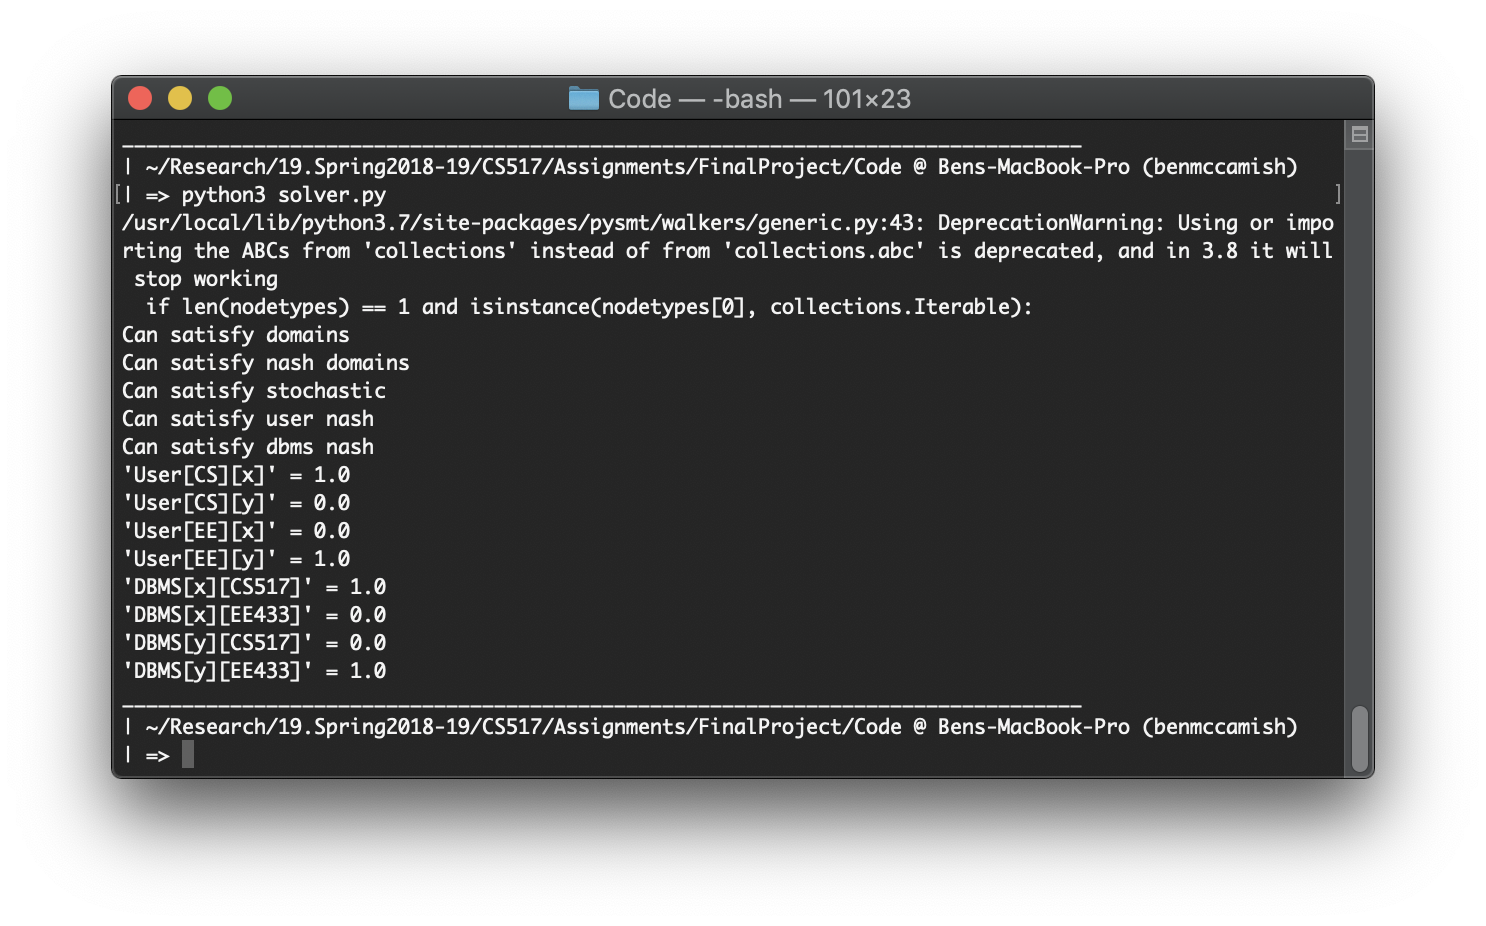
\includegraphics[width=20cm]{images/strictPaper}
\label{fig:strictpaper}
\caption{Strict Nash Solution}
\end{figure}

We can see that any deviation from this strategy will lead to a lower payoff. However, notice that the assignments are opposite of the one used in the example in the paper. This of course has the same payoff. The strategies can only reach that one by making two moves, where the first one will receive a lower payoff. This is the main point behind Strict Nash equilibria, as there is no incentive for either player to change their strategy since any move gets them a smaller payoff. There may be other Strict Nash equilibria that exist, however the players will not reach them from this strategy.

\begin{table}[h!]
    \centering
    \begin{minipage}{.2\linewidth}
        \caption{User strategy}
        \centering
        \begin{tabular}{c|c|c|}
            \cline{2-3}
             & \multicolumn{1}{c|}{$x$} & $y$\\
            \hline
            \multicolumn{1}{|c|}{``CS''} & 1 & 0\\
            \hline
            \multicolumn{1}{|c|}{``EE''} & 0 & 1\\
            \hline
        \end{tabular}
        \label{strictpaper:strategies:sender}
    \end{minipage}
    \begin{minipage}{.35\linewidth}
        \caption{DBMS strategy}
        \centering
        \begin{tabular}{c|c|c|}
            \cline{2-3}
             & \multicolumn{1}{c|}{``CS517''} & ``EE533''\\
            \hline
            \multicolumn{1}{|c|}{$x$} & 1 & 0\\
            \hline
            \multicolumn{1}{|c|}{$y$} & 0 & 1\\
            \hline
        \end{tabular}
        \label{strictpaper:strategies:receiver}
    \end{minipage}
       \begin{minipage}{.3\linewidth}
        \caption{Reward Matrix}
        \centering
        \begin{tabular}{c|c|c|}
            \cline{2-3}
             & \multicolumn{1}{c|}{``CS517''} & ``EE533''\\
            \hline
            \multicolumn{1}{|c|}{``CS''} & 1 & 0\\
            \hline
            \multicolumn{1}{|c|}{``EE''} & 0 & 1\\
            \hline
        \end{tabular}
        \label{strictpaper:strategies:reward}
    \end{minipage}
\end{table}

\subsection{Nash Example From Paper}
Keeping the current settings lets look at the output when we test on just a Nash equilibria. We can see the output in Figure~\ref{fig:paper}. We have materialized this into a strategy again for easier viewing in Tables~\ref{paper:strategies:sender},\ref{paper:strategies:receiver}, and~\ref{paper:strategies:reward}. 

\begin{figure}[h!]
\centering
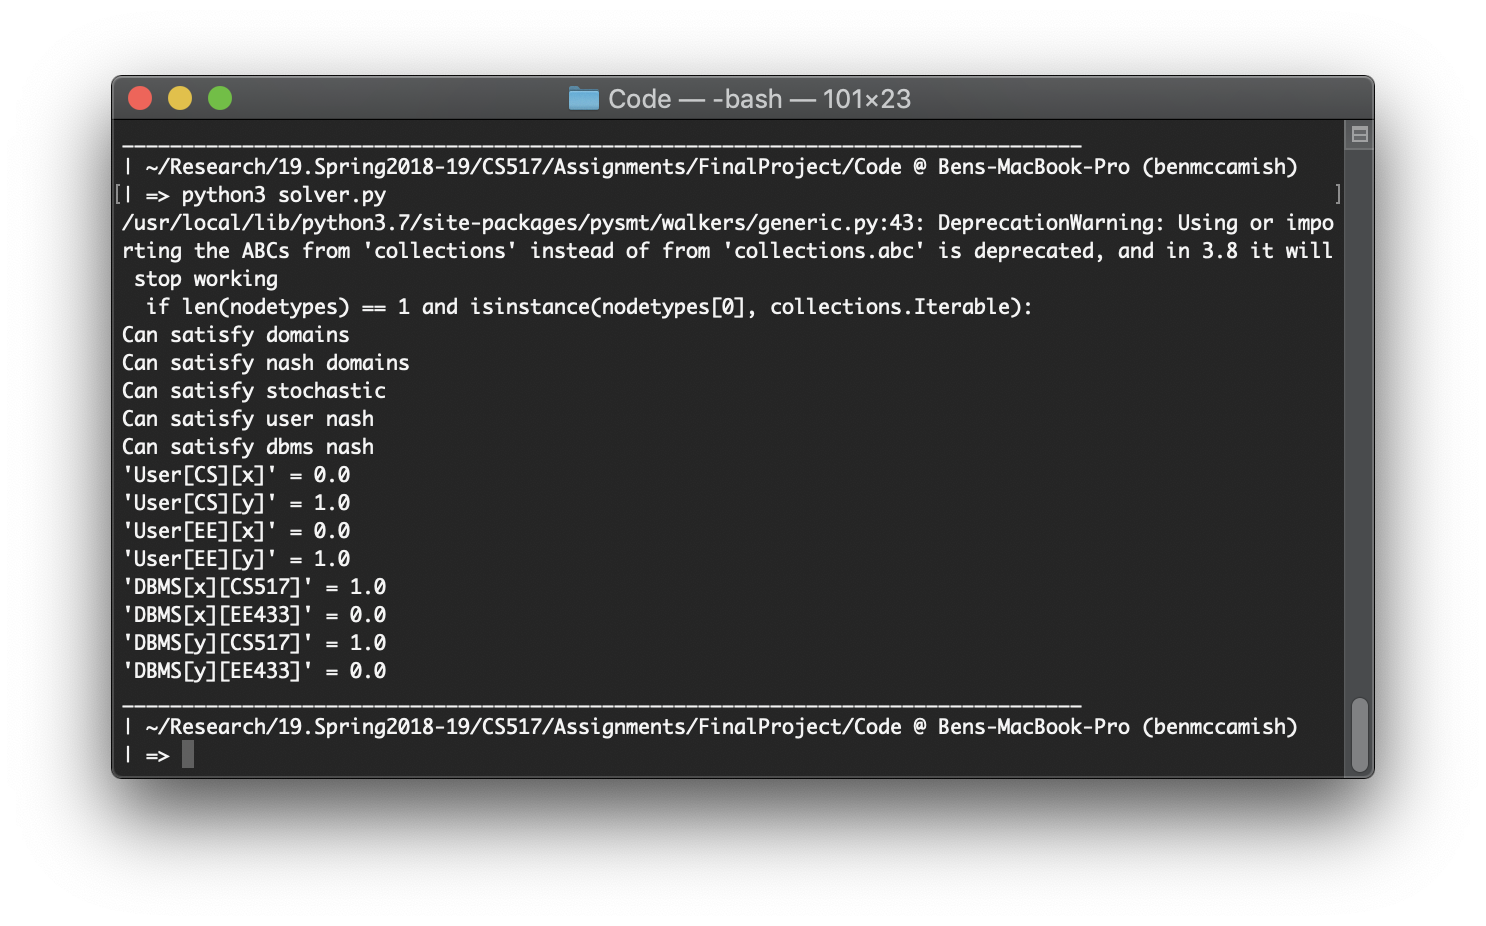
\includegraphics[width=20cm]{images/nashPaper}
\label{fig:paper}
\caption{Strict Nash Solution}
\end{figure}

This is a good example of a Nash equilibria. It is obviously not the best payoff we know we can receive from this setting. However, any single move that either player makes will result in a lesser or equal payoff. For example, no matter what query the user sends for ``EE'', it will always receive ``CS517''. If the DBMS decides to return ``EE433'' for the query ``y'', then the EE intent is satisfied, but now the CS intent is not satisfied. Again, a better strategy could be met by making multiple moves, but there is no incentive for the user or the DBMS to do this, as all the payoffs are the same or less. 

\begin{table}[h!]
    \centering
    \begin{minipage}{.2\linewidth}
        \caption{User strategy}
        \centering
        \begin{tabular}{c|c|c|}
            \cline{2-3}
             & \multicolumn{1}{c|}{$x$} & $y$\\
            \hline
            \multicolumn{1}{|c|}{``CS''} & 0 & 1\\
            \hline
            \multicolumn{1}{|c|}{``EE''} & 0 & 1\\
            \hline
        \end{tabular}
        \label{paper:strategies:sender}
    \end{minipage}
    \begin{minipage}{.35\linewidth}
        \caption{DBMS strategy}
        \centering
        \begin{tabular}{c|c|c|}
            \cline{2-3}
             & \multicolumn{1}{c|}{``CS517''} & ``EE533''\\
            \hline
            \multicolumn{1}{|c|}{$x$} & 1 & 0\\
            \hline
            \multicolumn{1}{|c|}{$y$} & 1 & 0\\
            \hline
        \end{tabular}
        \label{paper:strategies:receiver}
    \end{minipage}
       \begin{minipage}{.3\linewidth}
        \caption{Reward Matrix}
        \centering
        \begin{tabular}{c|c|c|}
            \cline{2-3}
             & \multicolumn{1}{c|}{``CS517''} & ``EE533''\\
            \hline
            \multicolumn{1}{|c|}{``CS''} & 1 & 0\\
            \hline
            \multicolumn{1}{|c|}{``EE''} & 0 & 1\\
            \hline
        \end{tabular}
        \label{paper:strategies:reward}
    \end{minipage}
\end{table}

Running the encoding of the SMT in Python was fairly fast for small strategies. As soon as I increased the size of intents, queries, and tuples to more than a couple dozen, it takes an incredibly long time. However, PySMT uses Cython so I was able to get that installed and working which I believe improved running times. 

\bibliographystyle{abbrv}
\bibliography{bib}

\end{document}
